\begin{figure}[H]
\centering
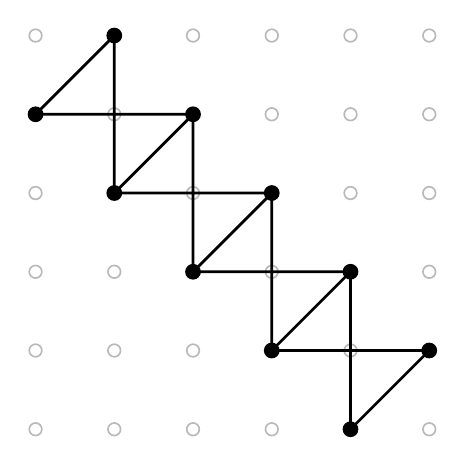
\begin{tikzpicture}[line cap=round, line join=round]

\foreach \x in {0,...,5} {
    \foreach \y in {0,...,5} {
    \draw[gray!55, line width=0.6pt] (\x,\y) circle[radius=0.08];
    }
}

\draw[black, line width=1.0pt]
    (0,4)--(1,5)
    (1,5)--(1,4)
    (0,4)--(1,4)--(2,4)
    (1,4)--(1,3)
    (1,3)--(2,4)
    (1,3)--(2,3)--(2,4)
    (2,3)--(2,2)
    (2,3)--(3,3)
    (2,2)--(3,3)
    (2,2)--(3,2)--(3,3)
    (3,2)--(3,1)
    (3,2)--(4,2)
    (3,1)--(4,2)
    (3,1)--(4,1)--(4,2)
    (4,1)--(4,0)
    (4,1)--(5,1)
    (4,0)--(5,1);

\foreach \p in {(0,4),(1,5),(1,3),(2,4),(2,2),(3,3),(3,1),(4,2),(4,0),(5,1)}{
    \fill[black] \p circle[radius=0.10];
}
\end{tikzpicture}
\caption{A $\Grid_{2 \times 5}$ in a $\CGrid_{6 \times 6}$.}
\label{fig:two-wide-grid-in-cgrid}
\end{figure}